\section{Motivation}
Heutige Software wird üblicherweise so gebaut, dass sie funktioniert. Das bedeutet, dass eine Person, welche mit der Software interagiert, diese möglichst problemfrei nutzen kann. Dabei spielt oftmals vor alle in sicherheitskritischen Bereichen die Qualität eine große Rolle.
Um diese zu gewährleisten, werden verschiedenste Methoden wie zum Beispiel Unit-Tests, Integrationstests und manuelles Testen eingesetzt.\\
Ein Problem bei dieser Art Software zu testen ist allerdings, wenn Fälle außerhalb der bereits bekannten Tests aufkommen. Dies könnte für die jeweilige Software bedeuten, dass es zu keinem Problem bis hin zu großen finanziellem oder auch menschlichem Schaden kommen kann.\\
Mathematisch und maschinell geprüfte Programme sollen diese Lücke in Zukunft schließen.


\begin{itemize}
	\item Normale Software wird so gebaut und evaluiert, sodass sie funktioniert
	\item “If you start with an English-language specification, you’re inherently starting with an ambiguous specification,” said Jeannette Wing, corporate vice president at Microsoft Research. “Any natural language is inherently ambiguous. In a formal specification you’re writing down a precise specification based on mathematics to explain what it is you want the program to do.”
	\item \url{https://www.quantamagazine.org/formal-verification-creates-hacker-proof-code-20160920/}
	\item Fehler 40
	\item Was wenn ein Compiler auf unterschiedlichen System aus dem selben Sourcecode unterschiedliche Runnables macht?
	\item \url{https://www.mikrocontroller.net/articles/Compilerfehler}
	\item \url{https://blog.regehr.org/archives/26}
	\item Unit tests schreiben, um möglichst viele Fehler zu finden -> Proof Assistent um für alle korrekt zu funktionieren
	\item Proof Assistent benutzen um formal richtigen Code zu schreiben/generieren
	\item \textbf{Fragestellung: Wie gewährleiste ich sichereren/gut getesteten Code?}
\end{itemize}


\section{Grundlagen}
\subsection{Was ist ein Proof Assisstant}
\url{https://www.youtube.com/watch?v=95VlaZTaWgc&t=2646s}


\subsubsection{Proof Verifier}
\subsubsection{Theorem Provers}

\subsection{Übersicht}
\url{https://en.wikipedia.org/wiki/Proof_assistant}
\begin{itemize}
	\item ACL2
	\item Isabelle
	\item Coq
\end{itemize}

\section{Coq}
\url{https://www.amazon.de/Certified-Programming-Dependent-Types-Introduction/dp/0262026651/ref=sr_1_fkmr0_1?__mk_de_DE=ÅMÅŽÕÑ&keywords=coq+proof+assistent&qid=1572974699&sr=8-1-fkmr0}
\begin{itemize}
	\item Warum Coq
	\item funktionaler Programmierstil
	\item Frenchmade
	\item Warum ist coq so erfolgreich?
\end{itemize}

\section{Programmatische Coq-Grundlagen}
\begin{itemize}
	\item Dependent type Sprache: So we established that we can prove things are true before we have a concrete value. To do this in an actual programming language, we need a way to encode these statements into the type system itself, which means our type system needs an upgrade. \url{https://medium.com/background-thread/the-future-of-programming-is-dependent-types-programming-word-of-the-day-fcd5f2634878}
	We're turning the above run-time assertion into compile-time type.
	\item \url{https://softwarefoundations.cis.upenn.edu/lf-current/Basics.html#lab18}
\end{itemize}
\subsection{Basisbegriffe}
\subsubsection{Typdefinition}
\begin{lstlisting}[language=coq,firstnumber=1,caption=Coq Typedefinition,label=lst:typedefinition]
Inductive bool : Type :=
	| true
	| false.
	
Inductive day : Type :=
	| monday
	| tuesday
	| wednesday
	| thursday
	| friday
	| saturday
	| sunday.
	
Inductive nat : Type :=
	| O
	| S (n : nat).
\end{lstlisting}

Die Beispiele aus dem Codeblock \ref{lst:typedefinition} stellen drei Typedefinitionen in Coq dar. Ersteres ist ein klassischer Bool. Sowie dieser true oder false annehmen kann, repräsentiert der zweite Type day alle Wochentage. \\
Die letzte Definition wird verwendet um alle natürlichen Zahlen darzustellen. \textbf{S (n : nat)} stellt den Successor z.d. die Nachfolgefunktion dar. Somit kann durch diesen Typ jeder Zahlenwert der natürlichen Zahlen dargestellt werden. Eine 4 würde beispielsweise durch die vierte Nachfolgefunktion von 0 wie folgt dargestellt werden. \textbf{(S (S (S (S O)))) => 0 + 1 + 1 + 1 + 1 => 4}.\\
Des Weiteren ist es auch möglich Komposition durch das Schlüsselwort \textbf{Inductive} abzubilden.

\subsubsection{Funktionen}
In Coq gibt es mehrere Arten von Funktionstypen. Mit dem Keyword \textbf{Definition} können einfach Funktionen dargestellt werden. Oftmals wird allerdings Rekursion benötigt. Diese ist nur möglich, wenn die Deklaration mit \textbf{Fixpoint} oder ähnlichen Wörtern beschrieben ist. Anstelle von \textbf{Theorem} könnten Beispielsweise auch \textbf{Example, Lemma, Fact oder Remark} stehen. Diese Schlüsselwörter ermöglichen es in Coq mittels des Allquantors die Korrektheit einer Funktion für alle Elemente einer Menge zu beweisen.
In Codeblock \ref{lst:functions} ist für die unterschiedlichen Funktionstypen jeweils ein Beispiel dargestellt.
\begin{lstlisting}[language=coq,firstnumber=1,caption=Coq Funktionen,label=lst:functions]
Definition minustwo (n : nat) : nat :=
match n with
	| O => O
	| S O => O
	| S (S n') => n'
end.

Theorem plus_O_n' : forall n : nat,
0 + n = n.

Fixpoint plus (n : nat) (m : nat) : nat :=
match n with
	| O => m
	| S n' => S (plus n' m)
end.
\end{lstlisting}

Die erste Funktion \textbf{minustwo} zieht von einer eingegebenen natürlichen Zahl zwei ab. Allerdings ergibt \textbf{0 - 2, 1 - 2 => 0}. Dies ist durch die ersten zwei Fälle des \textbf{match}-Begriffs dargestellt.\\
Das \textbf{Theorem plus\_O\_n} liest sich wie folgt: "Für alle natürlichen Zahlen n gilt 0 + n = 0". In folgendem Kapitel wird gezeigt, wie eine solche Funktion mathematisch bewiesen werden kann.

\begin{lstlisting}[language=coq,firstnumber=1,caption=Coq rekursive Funktion,label=lst:functions-executed]
(* Run function plus with 3 and 2. Result => 5 *)
Compute (plus 3 2).

(*  plus (S (S (S O))) (S (S O))
	==> S (plus (S (S O)) (S (S O)))
by the second clause of the match
	==> S (S (plus (S O) (S (S O))))
by the second clause of the match
	==> S (S (S (plus O (S (S O)))))
by the second clause of the match
	==> S (S (S (S (S O))))
by the first clause of the match
*)
\end{lstlisting}
Um ein tieferes Verständnis für die Rekursion in Coq zu bekommen, sind im Codeblock \ref{lst:functions-executed} die einzelnen Schritte abgebildet. Im 1. Schritt stellt Coq, wie bereits bei den Typdefinitionen der natürlichen Zahlen gezeigt, die Dezimalzahlen zwei und drei mittels der Successor-funktion dar. Anschließend beginnt die Rekursion. Solange \textbf{n > 0}, wird 1 mehr zum Endergebnis gezählt. Wenn \textbf{n = 0}, dann wird, wie in den letzten zwei Zeilen im Codeblock dargestellt, das plus durch \textbf{m} ersetzt. Somit ergibt \textbf{plus 3 2 => 5}.

\subsection{Beweise}
\subsubsection{Taktik}
\subsubsection{Ziele und Subgoals}
\subsubsection{Beispielbeweise}

\begin{lstlisting}[language=coq,firstnumber=1,caption=Coq Beispielbeweis,label=lst:sample-proof1]
(* Initiating the theorem to proof. *)
Theorem plus_id_exercise : forall n m o : nat,
	n = m ->
	m = o ->
	n + m = m + o.
	
(* result: 
1 subgoal
______________________________________(1/1)
forall n m o : nat,
n = m -> m = o -> n + m = m + o*)

Proof.
(* move quantifiers into the context: *)
	intros n m o. 
	
(* result: 
1 subgoal
n, m, o : nat
______________________________________(1/1)
n = m -> m = o -> n + m = m + o*)

(* move hypothesises into the context: *)	
	intros H.
	intros H2.

(* result: 
1 subgoal
n, m, o : nat
H : n = m
H2 : m = o
______________________________________(1/1)
n + m = m + o*)

(* rewrite the goal using the hypothesises: *)
	rewrite -> H.

(* result: 
...
______________________________________(1/1)
m + m = m + o
*)
	rewrite <- H2.

(* result:
...
______________________________________(1/1)
m + m = m + m
*)
	reflexivity.
Qed.
\end{lstlisting}

\section{Zusammenspiel Proof - Program}
\begin{itemize}
	\item Wir haben eine Liste von Dingen, die die Software tun soll, und verwenden Logik, um zu beweisen, dass die Software diese Dinge tut.
	\item \url{https://www.youtube.com/watch?v=Ue8QG8pf0wU}
	\item Codegenerierung, Proof -> Program
	\item Programm -> Proof
	\item Beispiel mit Liste aus Video
\end{itemize}

\subsection{How-to}
\begin{itemize}
	\item \url{https://medium.com/@ahelwer/formal-verification-casually-explained-3fb4fef2e69a}
	\item Erstelle eine Spezifikation, die ein Programm beschreibt
	\item Schreie die Spezifikation mathematisch in ein Proof Tool
	\item Wenn es Fehler enthält, sagt es dir der Verifier
	\item 
\end{itemize}

\section{Aktuelle Anwendung}
\subsection{Proofed Stack}
\begin{itemize}
	\item CompCert (C compiler)
	\item Princeton VST
	\item Certikos (verified Operating System with hypervisor and multi instances)
	\item \url{http://plv.csail.mit.edu/kami/}
	\item \url{https://www.zdnet.com/article/certikos-a-hacker-proof-os/}
	\item \url{https://github.com/PrincetonUniversity/VST}
	\item \url{https://vst.cs.princeton.edu}
	\item \url{https://news.yale.edu/2016/11/14/certikos-breakthrough-toward-hacker-resistant-operating-systems}
\end{itemize}
\subsection{CompCert for C}
\url{http://compcert.inria.fr}
\subsection{JSCert for ECMA 5}
\url{https://github.com/jscert/jscert}
\subsection{4-Farben Rätsel ist löstbar!}
\subsection{CertiCoq}
\url{https://www.cs.princeton.edu/~appel/papers/certicoq-coqpl.pdf}

\section{Anwendbarkeit in der Praxis}
\begin{itemize}
	\item Objektorientierung
	\item Sicherheitskritische Systeme
	\item Compilerbau
\end{itemize}


\section{Fazit}
\subsection{Aussicht}

\section{Glossar}


\section{Einleitung}
\label{s:intro}

Hier kommt die Einleitung.


%%%%%%%%%%%%%%%%%%%%%%%%%%%%%%%%%%%%%%%%%%%%%%%%%%%%%%%%%%%%%%
\subsection{Ein Abschnitt der Einleitung}
\label{ss:intro:abc}

Einen Überblick findet man z.\,B.\ in \cite{Auer00:HTF}.

\begin{figure}[t]
	\centering
	
	\begin{subfigure}{0.45\linewidth}
		\centering
		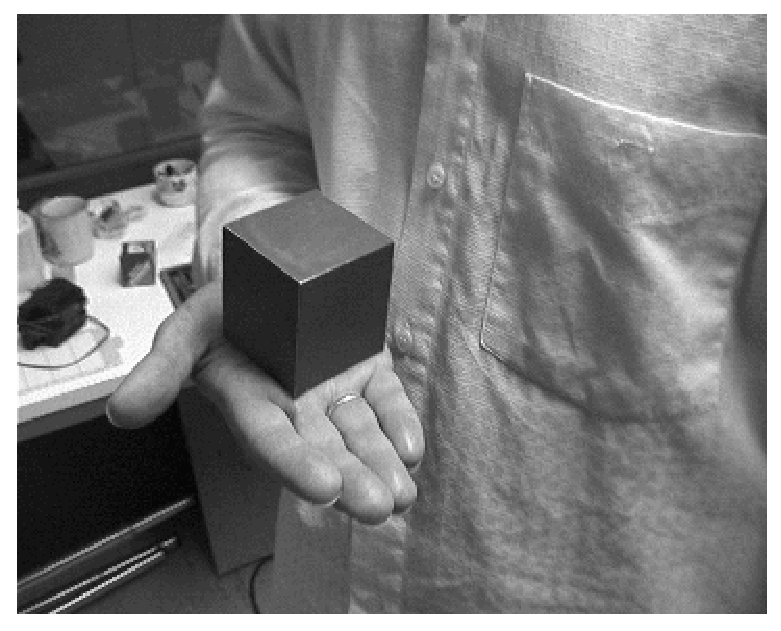
\includegraphics[width=\linewidth]{\figdir/handorig}
		\caption{Originalbild}
		\label{FIG:arexorig}
	\end{subfigure}
	%
	\begin{subfigure}{0.45\linewidth}
		\centering
		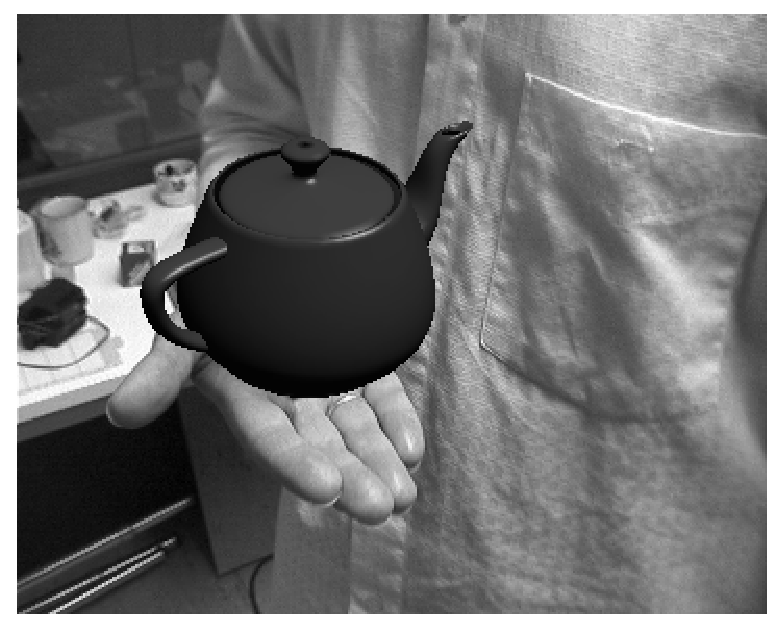
\includegraphics[width=\linewidth]{\figdir/handaug}
		\caption{erweitertes Bild}
		\label{FIG:arexaugm}
	\end{subfigure}
	%
	\caption[AR Beispiel]
	{Beispiel eines Augmented Reality Systems: es folgt eine Beschreibung (Bilder aus \cite{Schmidt01:PAO})}
	\label{FIG:arex}
\end{figure}

Ein Beispiel wird in Abb.\ \ref{FIG:arex} gezeigt.
Das verwendete Objekt ist in Abb.\ \ref{FIG:arexorig} dargestellt, das Ergebnis in Abb.\ \ref{FIG:arexaugm}.

Eine Formel
\begin{equation}
\label{eq:cvp:test}
f(x) = \frac{1}{3} x + 5, \quad x \in \real.
\end{equation}

Und noch eine:
\begin{equation}
\label{eq:cvp:matvec}
\bm{M}  = \bm{Ax} \pi, \quad \bm{A} \in \real^{2 \times 2}, \bm{x} \in \real^2.
\end{equation}

Tabelle \ref{t:CodebookOverview} gibt einen Überblick über XYZ.

\begin{table}[t]
	\centering\small
	%
% generated by TexTableGenerator.pl ((c) Florian Vogt)
% from file: /home/Jochen/data/dissdata/results/CodebookOverview.log
%
\begin{tabular}{l|ccc|cc}
\hline
\hline
                  \textbf{Sequence} &          ARTS &           wman &         stcams &         ARTVZ &        ARTSUZ \\ 
                 \textbf{\# Frames} &             190 &              40 &             400 &             270 &             190 \\ 
     \textbf{\# relative movements} &           17955 &             780 &           79800 &           36315 &           17955 \\ 
\textbf{\# movements after pre-sel.} &           14336 &             623 &           37915 &           21788 &           14343 \\ 
       \textbf{min.\ angle in seq.} &   0.233$^\circ$ &    5.95$^\circ$ &   0.154$^\circ$ & 0.00000171$^\circ$ &  0.0388$^\circ$ \\ 
       \textbf{max.\ angle in seq.} &    81.7$^\circ$ &     180$^\circ$ &    47.3$^\circ$ &    80.3$^\circ$ &    80.9$^\circ$ \\ 
\textbf{min.\ angle after pre-sel.} &    12.9$^\circ$ &    21.1$^\circ$ &    17.3$^\circ$ &    16.3$^\circ$ &    12.9$^\circ$ \\ 
\textbf{max.\ angle after pre-sel.} &    81.7$^\circ$ &     161$^\circ$ &    47.3$^\circ$ &    80.3$^\circ$ &    80.9$^\circ$ \\ \hline\hline
\end{tabular}

	\caption[Testtabelle]{Datenselektion für verschiedene Testdatensätze.}
	\label{t:CodebookOverview}
\end{table}


%%% Local Variables: 
%%% mode: latex
%%% TeX-master: "thesis.tex"
%%% End: 
